\documentclass[a4paper,11pt]{report}
\usepackage[showexo=true,showcorr=false]{../packages/coursclasse}

\toggletrue{montrerNiveaux}

\usepackage{enumitem}
\setlist[enumerate]{align=left,leftmargin=1cm,itemsep=10pt,parsep=0pt,topsep=0pt,rightmargin=0.5cm}
\setlist[itemize]{align=left,labelsep=1em,leftmargin=*,itemsep=0pt,parsep=0pt,topsep=0pt,rightmargin=0cm}

\setlength\columnsep{20pt}

\begin{document}

\newcommand{\chapterName}{Nombres et opérations}
\newcommand{\serieName}{Les nombres entiers relatifs}

\chapter*{\chapterName}
\thispagestyle{empty}

\begin{amL}{\serieName}{
\item Nombres entiers relatifs (page 17)
\item Distance à zéro (page 17)
\item Droite numérique (page 11)
\item Ordre croissant et décroissant (page 11)
}
\end{amL}

\section*{\serieName}
\setcounter{page}{1}
\thispagestyle{firstPage}



\begin{QSJ}{39}{1}
\end{QSJ}
\begin{resolu}{Les relatifs au quotidien}{
Retrouve dans la liste ci-dessous à quelle situation correspond chacune de ces températures: 
\[+37;\quad\quad -18;\quad\quad   -50; \quad \quad +4\]
\begin{tasks}(2)
\task Un congélateur: $-18$;
\task Un frigo: $+4$;
\task Le corps humain: $+37$;
\task Un hiver en Sibérie: $-50$.
\end{tasks}}
{1}
\end{resolu}

\begin{exop}
{Explique pourquoi dans ce tableau on a utilisé des nombres précédés d'un signe positif ($+$) ou négatif ($-$).
\begin{center}
\begin{tabular}{|c||c||c||c|}
 \hline
  Equipe & Buts marqués &  Buts encaissés & Différence\\   
\hline
Monaco &    $41$  & $17$    & $+24$ \\
 \hline
Paris St-Germain &$30$&$22$&$+8$ \\
 \hline
Bordeaux  &$31$      & $29$    &    $+2$ \\ 
\hline
Sedan &$27$      &$28$     &$-1$ \\
\hline
Rennes& $26$     & $26$    &    $0$\\ 
 \hline     
Strasbourg &    $19$  & $27$    & $-8$\\
\hline  
\end{tabular}  
\end{center}
\vspace{-0.5cm}
\begin{center}
\tiny{Football: Extrait de la situation après la 19ème journée du championnat.}   
\end{center}
\vspace{-0.5cm}}
{1}
\end{exop}

\begin{exof}{NO114}{41}{1}
\end{exof}
\begin{exol}{NO110}{36}{1}
\end{exol}

\begin{exop}
{Retrouve dans la liste ci-dessous à quelle situation correspond chacune de ces températures:  
	\[-310; \quad \quad  0; \quad \quad +310\]
\begin{tasks}
	\task La température de solidificaton de l'eau en glace est $\hrulefill$ \tunit{}{\degreeCelsius}.
\task La profondeur maximale du lac Léman est de $\;$\hrulefill$\;$ mètres.
\task Casablanca est à \hrulefill
$\;$ mètres par rapport au niveau de la mer. 
\end{tasks}}
{1}
\end{exop}

\begin{exo}
{Parmi les nombres ci-dessous:
	\[2;\quad \quad 3,5;\quad \quad -4,7;\quad \quad -12\quad \quad 7,2\]
Quels nombres sont $\ldots$
\begin{tasks}
\task  des nombres positifs: \dotfill
\task  des nombres négatifs: \dotfill
\task  des nombres entiers négatifs: \dotfill
\task  des nombres relatifs: \dotfill
\end{tasks}}
{1}
\end{exo}

\begin{exof}{NO111}{40}{1}
\end{exof}
\begin{exol}{NO106}{35}{3}
\end{exol}

\newpage

\begin{exop}
 {Quelle est la température indiquée par chacun des thermomètres~? 
\begin{multicols}{2}
\begin{tikzpicture}[y=0.5pt, x=0.5pt, yscale=-1, scale=0.7,inner sep=0pt, outer sep=0pt]
\foreach \y/\x in {190/100,227/80,264/80,301/60,338/40,375/20,412/0,449/$-20$,486/$-40$,523/$-60$,560/$-80$}
\draw (210,\y)--(190,\y) node[left](C\x){\x\tunit{}{\degreeCelsius}};
\path[draw=black,fill=white,miter limit=4,even odd rule,line width=2.5pt,fill=gray!20]
   [thermometer][path picture={\fill[red] (C40) rectangle (path picture bounding box.south east);}];
\draw (200,190)node[yshift=4ex] {Celsius} --(200,560) ;  
\end{tikzpicture}

\begin{tikzpicture}[y=0.5pt, x=0.5pt,yscale=-1,scale=0.7, inner sep=0pt, outer sep=0pt]
\foreach \y/\x in {190/30,227/25,264/20,301/15,338/10,375/5,412/0,449/$-5$,486/$-10$,523/$-15$,560/$-20$}
  \draw (210,\y)--(190,\y) node[left](C\x){\x\tunit{}{\degreeCelsius}};
\path[draw=black,fill=white,miter limit=4,even odd rule,line width=2.5pt,fill=gray!20]
   [thermometer][path picture={\fill[red] (C$-5$) rectangle (path picture bounding box.south east);}];
\draw (200,190)node[yshift=4ex] {Celsius} --(200,560) ; 
\end{tikzpicture}
\end{multicols}
\begin{tasks}(2)
	\task \dotfill \tunit{}{\degreeCelsius}
	\task \dotfill \tunit{}{\degreeCelsius}
\end{tasks}}
{1}
\end{exop}

%\begin{resolu}{La droite graduée 1}{
%Reprenons le premier thermomètre de l'exercice précédent et plaçons-le horizontalement. Nous pouvons remplacer ce thermomètre horizontal par une droite graduée. Le nombre en caractère gras est-il le même que la température indiquée par le thermomètre~?  
%    \begin{center}
%    \includegraphics[width=12cm]{media/thermomètre.pdf}
%
%    \begin{tikzpicture}[scale=0.9]
%  \draw[<->,ultra thick] (-8.2,0) -- (8.2,0);
%  \foreach \i in {-300,-250,...,340} % numbers on line
%    \draw ({8*\i/350},0.2) -- + (0,-0.4) node[below] {}; % tick and their labels
%  \draw ({8*(-300)/350},0.2) -- + (0,-0.4) node[below] {-100};
%  \draw ({8*(-50)/350},0.2) -- + (0,-0.4) node[below] {0};
%  \draw ({8*(50)/350},0.2) -- + (0,-0.4) node[below] {\color{red}{\textbf{40}}};
%  \draw ({8*(100)/350},0.2) -- + (0,-0.4) node[below] {60};
%  \foreach \i in {-340,-330,...,340} % numbers on line
%    \draw ({8*\i/350},0.1) -- + (0,-0.1) node[below] {}; % tick and their labels
%    \end{tikzpicture}
%\end{center}
\vspace{-0.5cm}
%
%{ La température indiquée sur le thermomètre est la même que celle indiquée sur la droite graduée (40 degrés). Une droite graduée peut ainsi se lire comme un thermomètre.}
%}{1}
%\end{resolu}

\begin{resolu}{La droite graduée}{
Place les nombres suivants sur la droite graduée: $-310; \quad 0;\quad +310$.
\begin{center}
	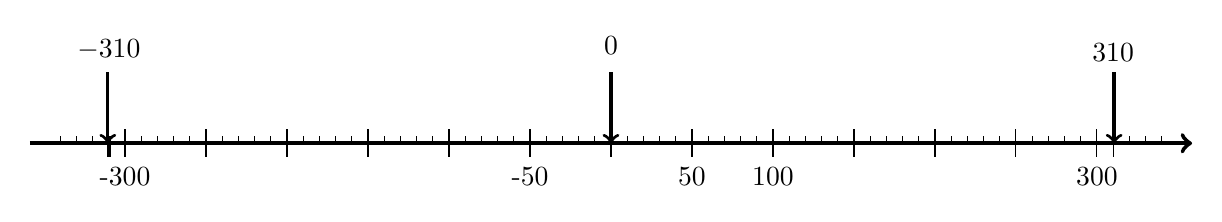
\begin{tikzpicture}[scale=0.9]
  \draw[->,ultra thick] (-8.2,0) -- (8.2,0);
  \foreach \i in {-300,-250,...,340} % numbers on line
    \draw ({8*\i/350},0.2) -- + (0,-0.4) node[below] {}; % tick and their labels
  \draw ({8*(-300)/350},0.2) -- + (0,-0.4) node[below] {-300};
  \draw ({8*(-50)/350},0.2) -- + (0,-0.4) node[below] {-50};
  \draw ({8*(50)/350},0.2) -- + (0,-0.4) node[below] {50};
  \draw ({8*(100)/350},0.2) -- + (0,-0.4) node[below] {100};
  \draw ({8*(300)/350},0.2) -- + (0,-0.4) node[below] {300};
  \foreach \i in {-340,-330,...,340} % numbers on line
    \draw ({8*\i/350},0.1) -- + (0,-0.1) node[below] {}; % tick and their labels

  % réponses
\draw[very thick][->] (-7.1,1) -- (-7.1,0);
\draw[very thick][->] (0,1) -- (0,0);
\draw[very thick][->] (7.1,1) -- (7.1,0);
  \draw ({8*(0)/350},0.1) -- + (0,-0.1) node[above=1cm] {0};
 \draw[very thick] ({8*(-310)/350},0.1) -- + (0,-0.3) node[above=1.1cm] {$-$310};
 \draw ({8*(310)/350},0.1) -- + (0,-0.3) node[above=1.1cm] {310};
\end{tikzpicture}
\end{center}
\vspace{-0.5cm}
}
{1}
\end{resolu}

\begin{exol}{NO104}{34}{1}
\end{exol}
\begin{exol}{NO107}{35}{1}
\end{exol}
\newpage

\begin{exop}
{Retrouve dans la liste ci-dessous à quelle situation correspond chacune de ces dates, puis place-les sur la droite.  
\begin{center}
{{ $+1400$;\hspace{0.5 cm}  $-3300$;\hspace{0.5 cm} $+2000$;\hspace{0.5 cm} $-2700$}}
\end{center}
\vspace{-0.5cm}
\begin{tasks}[after-item-skip = 0.2em]
\task La construction des pyramides en Egypte: \dotfill
\task La sortie du premier smatphone: \dotfill
\task L'invention de l'écriture:\dotfill
\task L'invention de l'imprimerie:\dotfill
\end{tasks}

\begin{center}
	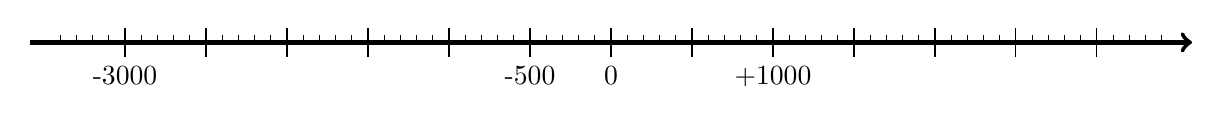
\begin{tikzpicture}[scale=0.9]
 \draw[->,ultra thick] (-8.2,0) -- (8.2,0);
  \foreach \i in {-300,-250,...,340} % numbers on line
    \draw ({8*\i/350},0.2) -- + (0,-0.4) node[below] {}; % tick and their labels
  \draw ({8*(-300)/350},0.2) -- + (0,-0.4) node[below] {-3000};
  \draw ({8*(-50)/350},0.2) -- + (0,-0.4) node[below] {-500};
  \draw ({8*(0)/350},0.2) -- + (0,-0.4) node[below] {0};
  \draw ({8*(100)/350},0.2) -- + (0,-0.4) node[below] {+1000};
  \foreach \i in {-340,-330,...,340} % numbers on line
    \draw ({8*\i/350},0.1) -- + (0,-0.1) node[below] {}; % tick and their labels
\end{tikzpicture}
\end{center}
\vspace{-0.5cm}
}
{1}
\end{exop}

%\begin{resolu}{Plus petit ou plus grand~?}{
%Complète le texte.
%Plus l'évènement est ancien, plus il est à .............................. sur la droite graduée. 
%Cela signifie aussi que le nombre est plus .............................. qu'un nombre plus ..............................qui est à ..............................}
%{1}
%\end{resolu}

\begin{exof}{NO102}{40}{1}
\end{exof}
\begin{exol}{NO103}{34}{1}
\end{exol}
\begin{exop}
{Place les points suivants sur la droite graduée.
\[A(+1); \quad \quad B(-3); \quad \quad C(0); \quad \quad D(+0,5)\]
\begin{center}
	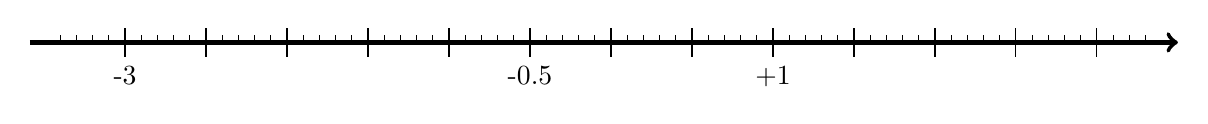
\begin{tikzpicture}[scale=0.9]
  \draw[->,ultra thick] (-8.2,0) -- (8.0,0);
  \foreach \i in {-300,-250,...,300} % numbers on line
    \draw ({8*\i/350},0.2) -- + (0,-0.4) node[below] {}; % tick and their labels
 \draw ({8*(-300)/350},0.2) -- + (0,-0.4) node[below] {-3};
  \draw ({8*(-50)/350},0.2) -- + (0,-0.4) node[below] {-0.5};
  \draw ({8*(100)/350},0.2) -- + (0,-0.4) node[below] {$+1$};
 \foreach \i in {-340,-330,...,330} % numbers on line
    \draw ({8*\i/350},0.1) -- + (0,-0.1) node[below] {}; % tick and their labels
\end{tikzpicture}
\end{center}
\vspace{-0.5cm}
}
{1}
\end{exop}

\begin{exop}
{Place les points suivants sur la droite graduée.
	\[A(+1,5);\quad B(-2);\quad C(+1,45);\quad D(+2,8);\quad E(+1,9);\quad F(-1,9)\]
	\begin{center}
		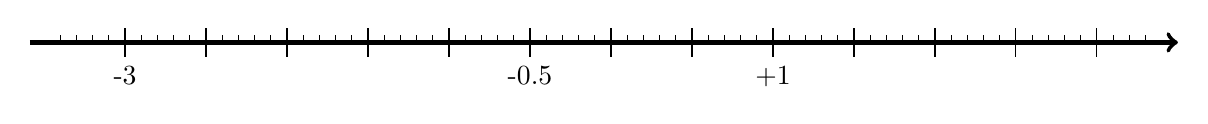
\begin{tikzpicture}[scale=0.9]
  \draw[->,ultra thick] (-8.2,0) -- (8.0,0);
  \foreach \i in {-300,-250,...,300} % numbers on line
    \draw ({8*\i/350},0.2) -- + (0,-0.4) node[below] {}; % tick and their labels
 \draw ({8*(-300)/350},0.2) -- + (0,-0.4) node[below] {-3};
  \draw ({8*(-50)/350},0.2) -- + (0,-0.4) node[below] {-0.5};
  \draw ({8*(100)/350},0.2) -- + (0,-0.4) node[below] {$+1$};
 \foreach \i in {-340,-330,...,330} % numbers on line
    \draw ({8*\i/350},0.1) -- + (0,-0.1) node[below] {}; % tick and their labels
\end{tikzpicture}
\end{center}
\vspace{-0.5cm}
}
{2}
\end{exop}



\begin{exop}
{Place les points $A, B, C$  et $D$ d'abscisse donnée sur la droite graduée.
	\[ A(0,15);\quad B(-0,1);\quad C(-0,35);\quad D(+0,55)\]
\begin{center}
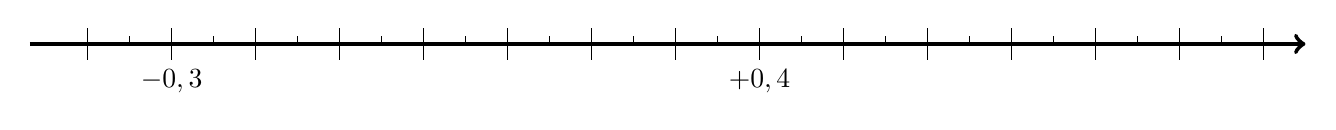
\begin{tikzpicture}
  \draw[->,ultra thick] (-8.2,0) -- (8.0,0);
  \foreach \i in {-700,-600,...,700} % numbers on line
    \draw ({8*\i/750},0.2) -- + (0,-0.4) node[below] {}; % tick and their labels
 \draw ({8*(-600)/750},0.2) -- + (0,-0.4) node[below] {$-0,3$};
  \draw ({8*(100)/750},0.2) -- + (0,-0.4) node[below] {$+0,4$};
 \foreach \i in {-650,-550,...,550,650} % numbers on line
    \draw ({8*\i/750},0.1) -- + (0,-0.1) node[below] {}; % tick and their labels
\end{tikzpicture}
\end{center}
\vspace{-0.5cm}
}
{2}
\end{exop}


\begin{exop}
{Détermine si les affirmations suivantes sont vraies ou fausses et corrige les affirmations fausses.

	\begin{tasks}
\task Il y a exactement deux entiers relatifs compris entre les points $C$ et $D$:\dotfill
\task La point $A$ a pour abscisse $+15$:\dotfill 
\task L'abscisse de $D$ est négative:\dotfill
\task L'origine de l'axe se situe au point $A$:\dotfill 
\end{tasks}
	\begin{center}
		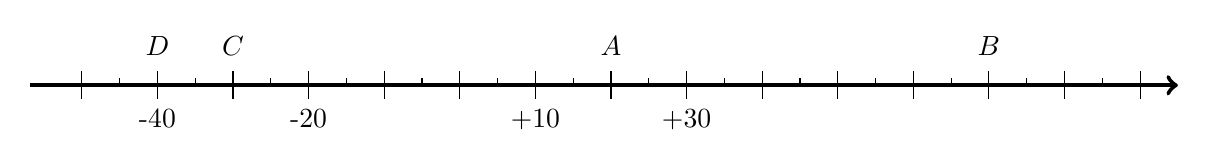
\begin{tikzpicture}[scale=0.9]
  \draw[->,ultra thick] (-8.2,0) -- (8.0,0);
  \foreach \i in {-700,-600,...,700} % numbers on line
    \draw ({8*\i/750},0.2) -- + (0,-0.4) node[below] {}; % tick and their labels
 \draw ({8*(-600)/750},0.2) -- + (0,-0.4) node[below] {-40};
 \draw ({8*(-400)/750},0.2) -- + (0,-0.4) node[below] {-20};
\draw ({8*(-100)/750},0.2) -- + (0,-0.4) node[below] {$+10$};
\draw ({8*(100)/750},0.2) -- + (0,-0.4) node[below] {$+30$};
 \foreach \i in {-650,-550,...,550,650} % numbers on line
    \draw ({8*\i/750},0.1) -- + (0,-0.1) node[below] {}; % tick and their labels
      \draw ({8*(0)/750},0.1) -- + (0,-0.1) node[above=0.25cm] {$A$};
  \draw ({8*(-500)/750},0.1) -- + (0,-0.1) node[above=0.25cm] {$C$};
    \draw ({8*(-600)/750},0.1) -- + (0,-0.1) node[above=0.25cm] {$D$};
  \draw ({8*(500)/750},0.1) -- + (0,-0.1) node[above=0.25cm] {$B$};
\end{tikzpicture}
\end{center}
\vspace{-0.5cm}
}
{2}
\end{exop}

\begin{exop}
{Donne les abscisses des points $A, B, C$ et $D$.

\begin{tasks}(2)
\task L'abscisse de $A$ est \points{2} 
\task L'abscisse de $B$ est \points{2}
\task L'abscisse de $C$ est \points{2}
\task L'abscisse de $D$ est \points{2}
\end{tasks}
	\begin{center}
		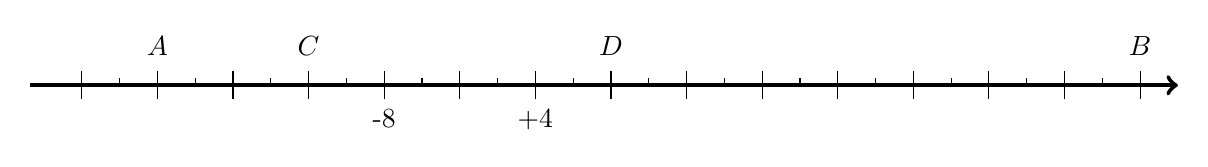
\begin{tikzpicture}[scale=0.9]
  \draw[->,ultra thick] (-8.2,0) -- (8.0,0);
  \foreach \i in {-700,-600,...,700} % numbers on line
    \draw ({8*\i/750},0.2) -- + (0,-0.4) node[below] {}; % tick and their labels
 \draw ({8*(-300)/750},0.2) -- + (0,-0.4) node[below] {-8};
\draw ({8*(-100)/750},0.2) -- + (0,-0.4) node[below] {$+4$};

 \foreach \i in {-650,-550,...,550,650} % numbers on line
    \draw ({8*\i/750},0.1) -- + (0,-0.1) node[below] {}; % tick and their labels
      \draw ({8*(0)/750},0.1) -- + (0,-0.1) node[above=0.25cm] {$D$};
  \draw ({8*(-400)/750},0.1) -- + (0,-0.1) node[above=0.25cm] {$C$};
    \draw ({8*(-600)/750},0.1) -- + (0,-0.1) node[above=0.25cm] {$A$};
  \draw ({8*(700)/750},0.1) -- + (0,-0.1) node[above=0.25cm] {$B$};
\end{tikzpicture}
\end{center}
\vspace{-0.5cm}
}
{2}
\end{exop}

\begin{exop}
{Donne les abscisses des points $A, B, C$ et $D$.
\begin{tasks}(2)
    \task L'abscisse de $A$ est: $\ldots\ldots\ldots$
     \task L'abscisse de $B$ est: $\ldots\ldots\ldots$
     \task L'abscisse de $C$ est: $\ldots\ldots\ldots$
     \task L'abscisse de $D$ est: $\ldots\ldots\ldots$
\end{tasks}

\begin{center}
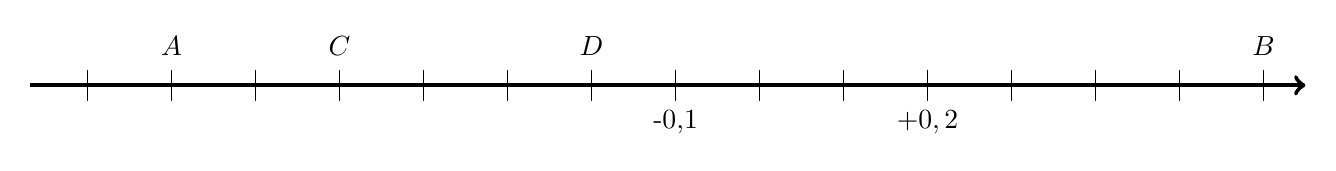
\begin{tikzpicture}
  \draw[->,ultra thick] (-8.2,0) -- (8.0,0);
  \foreach \i in {-700,-600,...,700} % numbers on line
    \draw ({8*\i/750},0.2) -- + (0,-0.4) node[below] {}; % tick and their labels
 \draw ({8*(0)/750},0.2) -- + (0,-0.4) node[below] {-0,1};
\draw ({8*(300)/750},0.2) -- + (0,-0.4) node[below] {$+0,2$};

      \draw ({8*(-100)/750},0.1) -- + (0,-0.1) node[above=0.25cm] {$D$};
  \draw ({8*(-400)/750},0.1) -- + (0,-0.1) node[above=0.25cm] {$C$};
    \draw ({8*(-600)/750},0.1) -- + (0,-0.1) node[above=0.25cm] {$A$};
  \draw ({8*(700)/750},0.1) -- + (0,-0.1) node[above=0.25cm] {$B$};
\end{tikzpicture}
\end{center}
\vspace{-0.5cm}
}
{3}
\end{exop}

\begin{exop}
{Donne les abscisses des points $A, B, C$ et $D$.
\begin{tasks}(2)
    \task L'abscisse de $A$ est: $\ldots\ldots\ldots$
     \task L'abscisse de $B$ est: $\ldots\ldots\ldots$
     \task L'abscisse de $C$ est: $\ldots\ldots\ldots$
     \task L'abscisse de $D$ est: $\ldots\ldots\ldots $
\end{tasks}

\begin{center}
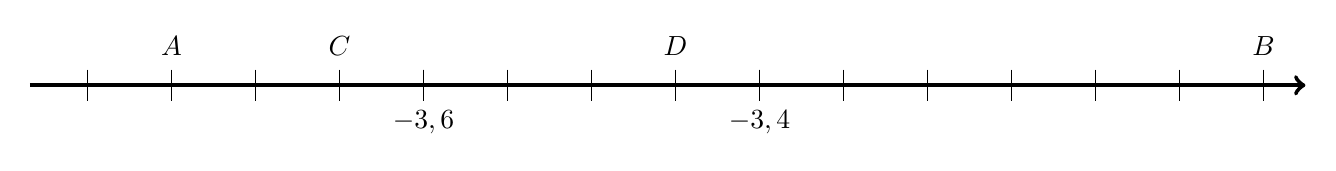
\begin{tikzpicture}
  \draw[->,ultra thick] (-8.2,0) -- (8.0,0);
  \foreach \i in {-700,-600,...,700} % numbers on line
    \draw ({8*\i/750},0.2) -- + (0,-0.4) node[below] {}; % tick and their labels
 \draw ({8*(-300)/750},0.2) -- + (0,-0.4) node[below] {$-3,6$};
\draw ({8*(100)/750},0.2) -- + (0,-0.4) node[below] {$-3,4$};

      \draw ({8*(0)/750},0.1) -- + (0,-0.1) node[above=0.25cm] {$D$};
  \draw ({8*(-400)/750},0.1) -- + (0,-0.1) node[above=0.25cm] {$C$};
    \draw ({8*(-600)/750},0.1) -- + (0,-0.1) node[above=0.25cm] {$A$};
  \draw ({8*(700)/750},0.1) -- + (0,-0.1) node[above=0.25cm] {$B$};
\end{tikzpicture}
\end{center}
\vspace{-0.5cm}
}
{3}
\end{exop}


\begin{resolu}{Comparaison}{Compare les nombres relatifs suivants en utilisant les signes $< ; > ;= $. Aide-toi de la droite graduée ci-dessous.

\begin{tasks}(4)
\task $-5 < +5$
\task $-5 > -6$
\task $0 > -3$
\task $0 < +5$
\end{tasks}

\begin{center}
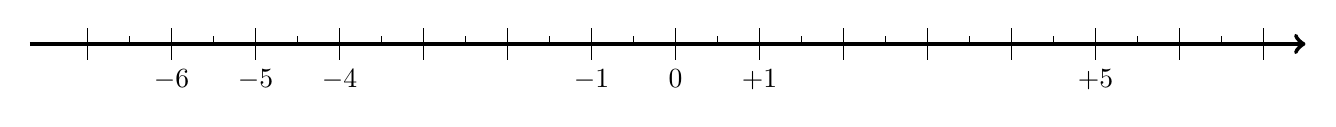
\begin{tikzpicture}
  \draw[->,ultra thick] (-8.2,0) -- (8.0,0);
  \foreach \i in {-700,-600,...,700} % numbers on line
    \draw ({8*\i/750},0.2) -- + (0,-0.4) node[below] {}; % tick and their labels
 \draw ({8*(-400)/750},0.2) -- + (0,-0.4) node[below] {$-4$};
  \draw ({8*(-100)/750},0.2) -- + (0,-0.4) node[below] {$-1$};
    \draw ({8*(100)/750},0.2) -- + (0,-0.4) node[below] {$+1$};
 \foreach \i in {-650,-550,...,550,650} % numbers on line
    \draw ({8*\i/750},0.1) -- + (0,-0.1) node[below] {}; % tick and their labels
      \draw ({8*(0)/750},0.1) -- + (0,-0.3) node[below] {$0$};
  \draw ({8*(-500)/750},0.1) -- + (0,-0.3) node[below] {$-$5};
    \draw ({8*(-600)/750},0.1) -- + (0,-0.3) node[below] {$-$6};
  \draw ({8*(500)/750},0.1) -- + (0,-0.3) node[below] {$+5$};
\end{tikzpicture}
\end{center}
\vspace{-0.5cm}
}
{1}
\end{resolu}


\begin{exop}
{Compare les nombres relatifs suivants en utilisant les signes  $< ; > ; =$. Aide-toi de la droite graduée ci-dessous.
\begin{tasks}[after-item-skip=0.2em](2)
\task $(+2)$ \ldots\ldots $(+5)$
\task $0$\ldots\ldots  $(+3)$
\task $0$ \ldots\ldots $(-4)$ 
\task $(-4)$ \ldots\ldots $(-2)$
\end{tasks}

\begin{center}
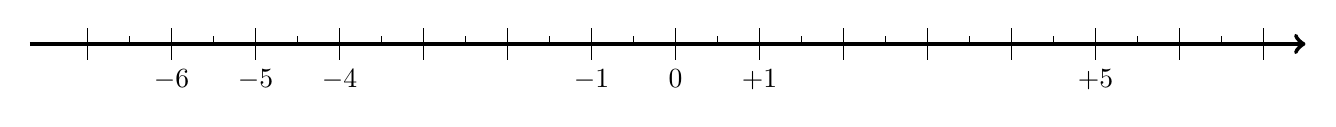
\begin{tikzpicture}
  \draw[->,ultra thick] (-8.2,0) -- (8.0,0);
  \foreach \i in {-700,-600,...,700} % numbers on line
    \draw ({8*\i/750},0.2) -- + (0,-0.4) node[below] {}; % tick and their labels
 \draw ({8*(-400)/750},0.2) -- + (0,-0.4) node[below] {$-4$};
  \draw ({8*(-100)/750},0.2) -- + (0,-0.4) node[below] {$-1$};
    \draw ({8*(100)/750},0.2) -- + (0,-0.4) node[below] {$+1$};
 \foreach \i in {-650,-550,...,550,650} % numbers on line
    \draw ({8*\i/750},0.1) -- + (0,-0.1) node[below] {}; % tick and their labels
      \draw ({8*(0)/750},0.1) -- + (0,-0.3) node[below] {$0$};
  \draw ({8*(-500)/750},0.1) -- + (0,-0.3) node[below] {$-$5};
    \draw ({8*(-600)/750},0.1) -- + (0,-0.3) node[below] {$-$6};
  \draw ({8*(500)/750},0.1) -- + (0,-0.3) node[below] {$+5$};
\end{tikzpicture}\end{center}
\vspace{-0.5cm}
}
{1}
\end{exop}

\begin{exop}
{Compare les nombres relatifs suivants en utilisant les signes $< ; > ; =$. Aide-toi de la droite graduée ci-dessous.
	\begin{tasks}[after-item-skip=0.2em](2)
	\task $(-2,5)$  \ldots\ldots $(-2)$
\task $(+3,5)$ \ldots\ldots $(+5)$ 
\task $(-3,5)$ \ldots\ldots $(+3)$
\task $(+0,5)$ \ldots\ldots $(-1,5)$
\end{tasks}
\begin{center}
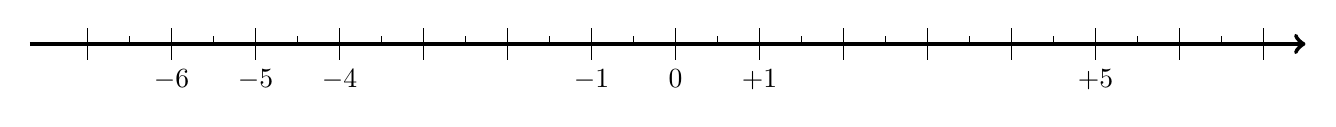
\begin{tikzpicture}
  \draw[->,ultra thick] (-8.2,0) -- (8.0,0);
  \foreach \i in {-700,-600,...,700} % numbers on line
    \draw ({8*\i/750},0.2) -- + (0,-0.4) node[below] {}; % tick and their labels
 \draw ({8*(-400)/750},0.2) -- + (0,-0.4) node[below] {$-4$};
  \draw ({8*(-100)/750},0.2) -- + (0,-0.4) node[below] {$-1$};
    \draw ({8*(100)/750},0.2) -- + (0,-0.4) node[below] {$+1$};
 \foreach \i in {-650,-550,...,550,650} % numbers on line
    \draw ({8*\i/750},0.1) -- + (0,-0.1) node[below] {}; % tick and their labels
      \draw ({8*(0)/750},0.1) -- + (0,-0.3) node[below] {$0$};
  \draw ({8*(-500)/750},0.1) -- + (0,-0.3) node[below] {$-$5};
    \draw ({8*(-600)/750},0.1) -- + (0,-0.3) node[below] {$-$6};
  \draw ({8*(500)/750},0.1) -- + (0,-0.3) node[below] {$+5$};
\end{tikzpicture}\end{center}
\vspace{-0.5cm}
}
{2}
\end{exop}

\begin{exof}{NO115}{41}{2}
\end{exof}
\begin{exop}
{Compare les nombres relatifs suivants en utilisant les signes $< ; > ; =$. 
\begin{tasks}[after-item-skip=0.2em](2)	
    \task $(-3)\ldots\ldots (-7)$
    \task $(+4)\ldots\ldots (+3)$
    \task $(-2)\ldots\ldots (+2)$
    \task $(-3)\ldots\ldots (+2)$
    \task $(-12)\ldots\ldots (-10)$
    \task $(+70)\ldots\ldots (-75)$
    \task $(-3)\ldots\ldots 0$
    \task $(+2)\ldots\ldots 0$
\end{tasks}
}
{1}
\end{exop}


\begin{exop}
{Compare les nombres relatifs suivants en utilisant les signes $< ; > ; =$.
	\begin{tasks}[after-item-skip=0.3em](2)	
    \task $(+4,5)$\ldots\ldots $(+4,45)$
    \task $(-4,5)$\ldots\ldots $(-4,45)$
    \task $(+0,1)$\ldots\ldots $(-10)$
    \task $(-0.5)$\ldots\ldots $0$
    \task $(+3,1)$\ldots\ldots $(+3,11)$
    \task $(-3,1)$\ldots\ldots $(-3,11)$
    \task $(-3,1)$\ldots\ldots $(+3,11)$
    \task $(+7,51)$\ldots\ldots $(-7,52)$
\end{tasks}
}
{2}
\end{exop}


%\begin{resolu}{Encadrement}{Complète ces lignes avec les 4 entiers relatifs manquants. Aide-toi de la droite graduée.
%
%\begin{tikzpicture}
%  \draw[<->,ultra thick] (-8.2,0) -- (8.0,0);
%  \foreach \i in {-700,-600,...,700} % numbers on line
%    \draw ({8*\i/750},0.2) -- + (0,-0.4) node[below] {}; % tick and their labels
% \draw ({8*(-400)/750},0.2) -- + (0,-0.4) node[below] {$-4$};
%  \draw ({8*(-100)/750},0.2) -- + (0,-0.4) node[below] {$-1$};
%    \draw ({8*(100)/750},0.2) -- + (0,-0.4) node[below] {$+1$};
% \foreach \i in {-650,-550,...,550,650} % numbers on line
%    \draw ({8*\i/750},0.1) -- + (0,-0.1) node[below] {}; % tick and their labels
%\draw ({8*(0)/750},0.1) -- + (0,-0.1) node[below] {0};
%  \draw ({8*(-500)/750},0.1) -- + (0,-0.3) node[below] {$-$5};
%    \draw ({8*(-600)/750},0.1) -- + (0,-0.3) node[below] {$-$6};
%  \draw ({8*(500)/750},0.1) -- + (0,-0.3) node[below] {$+5$};
%\end{tikzpicture}
%
%\begin{enumerate}
%    \item $(-3)$< {{$(-2) < (-1) < 0< (+1)$}}<$(+2)$
%    \item$(-5)$<
%    {{ $(-4) < (-3) < (-2) < (-1)$}}<$0$
%\end{enumerate}}
%{1}
%\end{resolu}

\begin{exop}
{Quels nombres entiers relatifs pourraient compléter ces lignes~?
	\begin{tasks}[after-item-skip=0.3em](2)		
\task $(-1)< \dotfill \medskip <(+5)$\hspace{0.3cm}
\task $(-5)<\dotfill \medskip <(+1)$    \hspace{0.3cm}
\task $(-15)<\dotfill \medskip <(-9)$\hspace{0.3cm}
\task $(-3)\dotfill \medskip <(+3)$\hspace{0.3cm}
\task $(-10) < \dotfill \medskip \leq(-3)$\hspace{0.3cm}
\task $(-6) < \dotfill \medskip \leq(-4)$\hspace{0.3cm}
	\end{tasks}
}{1}
\end{exop}

\begin{exof}{NO116}{42}{2}
\end{exof}


\begin{resolu}{Encadrement}{Encadre les nombres suivants par deux entiers consécutifs.
		\begin{tasks}[before-skip=-0.5em,after-skip=-0.5em](2)
			\task $(-2) \medskip <(-1,5)< \medskip (-1)$
\task $(+1) \medskip <(+1,75)< \medskip (+2)$
		\end{tasks}
}
{1}
\end{resolu}

\begin{exop}
{Encadre les nombres suivants par deux entiers consécutifs.
	\begin{tasks}[after-item-skip=0.2em,after-skip=-0.5em](2)		
		\task $\dotfill \medskip <(-2,5)< \medskip \dotfill$ \hspace{0.2cm}
\task $\dotfill \medskip <(-2,75)< \medskip \dotfill$\hspace{0.2cm}
\task $\dotfill \medskip <(-475,367)< \medskip \dotfill$\hspace{0.2cm}
\task $\dotfill \medskip <(+25,5)< \medskip \dotfill$\hspace{0.2cm}
	\end{tasks}
}
{2}
\end{exop}


\begin{resolu}{Ordre des relatifs}{Ordonne dans l'ordre croissant les nombres suivants en utilisant le signe approprié: $-10$; $+14$; $-8$; $-3$; $+4$; $+17$.
\[-10<-8<-3<+4<+14<+17\]
\vspace{-1cm}}
{1}
\end{resolu}

\begin{exol}{NO108}{35}{2}
\end{exol}
\begin{exol}{NO109}{36}{2}
\end{exol}

\begin{exop}
{\begin{tasks}[after-item-skip = 0.2em]
\task Ordonne dans l'ordre croissant les nombres suivants en utilisant le symbole "<" :  $+14$; $-7$; $+3$; $-8$; $+7$; $+8$; $-9$.

	\dotfill
\task Ordonne dans l'ordre croissant les nombres suivants en utilisant le symbole "<":  $-10$; $+14$; $-80$; $-380$; $+700$; $+87$; $-958$.

\dotfill
\task Ordonne dans l'ordre croissant les nombres suivants en utilisant le symbole approprié  $+5$; $+2,5$; $-2,5$; $-3,5$; $+7,5$; $-8,5$; $-0,2$.

	\dotfill
\task Ordonne dans l'ordre décroissant les nombres suivants en utilisant le symbole approprié:  $-10,6$; $+14,5$; $-8,3$; $-3,8$; $+4,2$; $+14,6$; $-8,3$.

	\dotfill
\task Ordonne dans l'ordre décroissant les nombres suivants en utilisant le symbole approprié: $-10,65$; $-10,70$; $-10,6$; $+3,85$; $+3,80$; $+3,9$;.

	\dotfill
\task Ordonne dans l'ordre croissant les nombres suivants en utilisant le symbole approprié:  $-10,6$; $+14,52$; $-8,31$; $+8,35$; $+4,2$;.

	\dotfill
\task Ordonne dans l'ordre croissant les nombres suivants en utilisant le symbole approprié:  $+5,35$; $-9,7$; $-12$; $+5,4$; $-9,790$; $+3,7$;.

	\dotfill
\end{tasks}}
{3}
\end{exop}

\begin{resolu}{ Valeur absolue}{
Pour chaque couple de nombres indique 
\begin{enumerate}[itemsep=5pt]
	\item[1)] celui qui a la plus grande valeur absolue;
	\item[2)] le plus grand des deux nombres.
\end{enumerate}
\begin{tasks}
    \task $M=(-12)$ et $N=(+6)$
    
    $M$ a la plus grande valeur absolue et $N$ est le plus grand des deux nombres.
    \task $M=(-8)$ et $N=(+10)$

     $N$ a la plus grande valeur absolue et est également le plus grand des deux nombres.
\end{tasks}}
{1}
\end{resolu}

\begin{exof}{NO102}{40}{1}
\end{exof}
\begin{exol}{NO109}{36}{1}
\end{exol}
\begin{exo}
{Pour chaque couple de nombres indique 
\begin{enumerate}[itemsep=5pt]
	\item[1)] celui qui a la plus grande valeur absolue;
	\item[2)] le plus grand des deux nombres.
\end{enumerate}
\begin{tasks}(2)
    \task $M=(+7)$ et $N=(-11)$
    \task $M= (+7)$ et $N=(-4)$
    \task $M= (+9)$ et $N=(-3)$
    \task $M= (-9)$ et $N=(-3)$
    \task $M= (-9)$ et $N=(+3)$
    \task $M= (+9)$ et $N=(+3)$
\end{tasks}}
{1}
\end{exo}

\begin{resolu}{Système d'axes}{Voici un système d'axes gradués.
Donne les coordonnées des points $A$ et $B$

\begin{minipage}[t]{0.6\textwidth}{
\vspace{0pt}
\begin{center}
	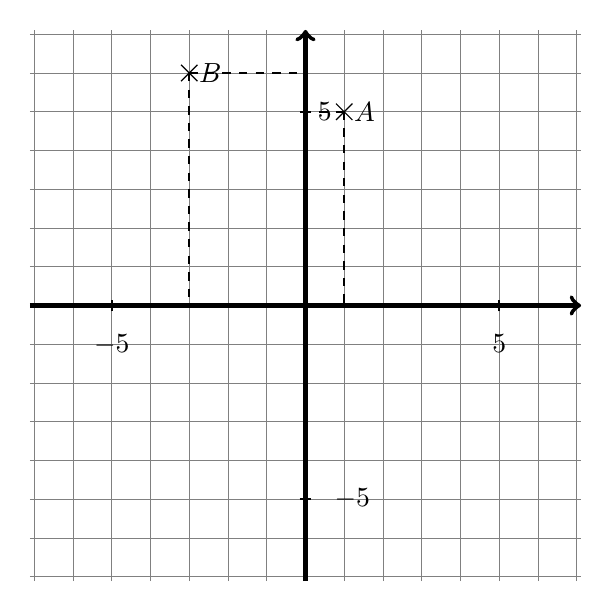
\begin{tikzpicture}[scale=0.7]
\draw[step= 20pt,gray,very thin](-5,-5) grid (5,5);

\coordinate (0) at (0,0);
\coordinate (1h) at (1,0);
\coordinate (2h) at (2,0);
\coordinate (3h) at (3,0);
\coordinate (4h) at (4,0);
\coordinate (5h) at (5,0);
\coordinate (6h) at (6,0);
\coordinate (-1h) at (-1,0);
\coordinate (-2h) at (-2,0);
\coordinate (-3h) at (-3,0);
\coordinate (-4h) at (-4,0);
\coordinate (-5h) at (-5,0);
\coordinate (-6h) at (-6,0);
\coordinate (1v) at (0,1);
\coordinate (2v) at (0,2);
\coordinate (3v) at (0,3);
\coordinate (4v) at (0,4);
\coordinate (5v) at (0,5);
\coordinate (6v) at (0,6);
\coordinate (-1v) at (0,-1);
\coordinate (-2v) at (0,-2);
\coordinate (-3v) at (0,-3);
\coordinate (-4v) at (0,-4);
\coordinate (-5v) at (0,-5);
\coordinate (-6v) at (0,-6);
\draw[ultra thick,->] (-5h) -- (5h);
\draw[ultra thick,->] (-5v) -- (5v);
\draw[thick] (100pt,-3pt) -- (100pt,3pt);
\draw[thick] (-100pt,-3pt) -- (-100pt,3pt);
\draw[thick] (-3pt,100pt) -- (3pt,100pt);
\draw[thick] (-3pt,-100pt) -- (3pt,-100pt);

\node[below] at (100pt,-10pt) {$5$};
\node[below] at (-100pt,-10pt) {$-5$};
%\node at (20pt,-10pt) {$\bm{1}$};
%\node at (-20pt,-10pt) {$\bm{-1}$};
\node at (10pt,100pt) {$5$};
\node[right] at (10pt,-100pt) {$-5$};

\filldraw (20pt,100pt)  node[anchor=west] {$A$};
\filldraw (-60pt,120pt) node[anchor=west] {$B$};
\draw plot[mark=x, mark options={ scale=3}] coordinates {(20pt,100pt) };
\draw plot[mark=x, mark options={ scale=3}] coordinates {(-60pt,120pt) };
\draw[thick,dashed] (20pt,100pt) -- (20pt,0);
\draw[thick,dashed] (20pt,100pt) -- (0,100pt);
\draw[thick,dashed] (-60pt,120pt) -- (-60pt,0);
\draw[thick,dashed] (-60pt,120pt) -- (0,120pt);
 \end{tikzpicture}
 \end{center}
\vspace{-0.5cm}
}
\end{minipage}
\begin{minipage}[t]{0.4\textwidth}{
\vspace{0pt}
 \begin{tasks}
     \task Les coordonnées du point $A$ sont: $(+1;+5)$.
     \task Les coordonnées du point $B$ sont: $(-3;+6)$.
 \end{tasks}
}\end{minipage}
}
 {1}
\end{resolu}

\newpage
\begin{exop}
{Voici un système d'axes gradués. 
	\vspace{-0.5cm}

\begin{minipage}[t]{0.5\textwidth}{
\vspace{0pt}
\begin{center}
	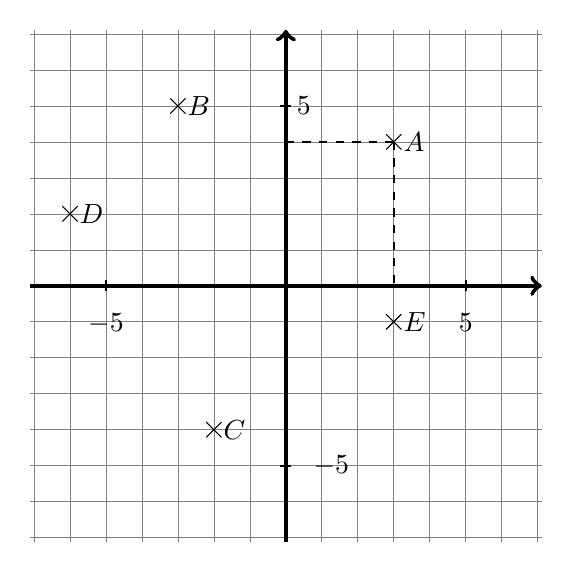
\begin{tikzpicture}[scale=0.65]
\draw[step= 20pt,gray,very thin](-5,-5) grid (5,5);

\coordinate (0) at (0,0);
\coordinate (1h) at (1,0);
\coordinate (2h) at (2,0);
\coordinate (3h) at (3,0);
\coordinate (4h) at (4,0);
\coordinate (5h) at (5,0);
\coordinate (6h) at (6,0);
\coordinate (-1h) at (-1,0);
\coordinate (-2h) at (-2,0);
\coordinate (-3h) at (-3,0);
\coordinate (-4h) at (-4,0);
\coordinate (-5h) at (-5,0);
\coordinate (-6h) at (-6,0);
\coordinate (1v) at (0,1);
\coordinate (2v) at (0,2);
\coordinate (3v) at (0,3);
\coordinate (4v) at (0,4);
\coordinate (5v) at (0,5);
\coordinate (6v) at (0,6);
\coordinate (-1v) at (0,-1);
\coordinate (-2v) at (0,-2);
\coordinate (-3v) at (0,-3);
\coordinate (-4v) at (0,-4);
\coordinate (-5v) at (0,-5);
\coordinate (-6v) at (0,-6);
\draw[ultra thick,->] (-5h) -- (5h);
\draw[ultra thick,->] (-5v) -- (5v);
\draw[thick] (100pt,-3pt) -- (100pt,3pt);
\draw[thick] (-100pt,-3pt) -- (-100pt,3pt);
\draw[thick] (-3pt,100pt) -- (3pt,100pt);
\draw[thick] (-3pt,-100pt) -- (3pt,-100pt);

\node[below] at (100pt,-10pt) {$5$};
\node[below] at (-100pt,-10pt) {$-5$};
%\node at (20pt,-10pt) {$\bm{1}$};
%\node at (-20pt,-10pt) {$\bm{-1}$};
\node at (10pt,100pt) {$5$};
\node[right] at (10pt,-100pt) {$-5$};

\filldraw (60pt,80pt)  node[anchor=west] {$A$};
\filldraw (-60pt,100pt)  node[anchor=west] {$B$};
\filldraw (-40pt,-80pt)  node[anchor=west] {$C$};
\filldraw (-120pt,40pt)  node[anchor=west] {$D$};
\filldraw (60pt,-20pt)  node[anchor=west] {$E$};
\draw plot[mark=x, mark options={ scale=3}] coordinates {(60pt,80pt) };
\draw plot[mark=x, mark options={ scale=3}] coordinates {(-60pt,100pt) };
\draw plot[mark=x, mark options={ scale=3}] coordinates {(-40pt,-80pt) };
\draw plot[mark=x, mark options={ scale=3}] coordinates {(-120pt,40pt) };
\draw plot[mark=x, mark options={ scale=3}] coordinates {(60pt,-20pt) };

\draw[thick,dashed] (60pt,80pt) -- (60pt,0);
\draw[thick,dashed] (60pt,80pt) -- (0,80pt);
 \end{tikzpicture}
\end{center}
\vspace{-0.5cm} 

}
\end{minipage}
\begin{minipage}[t]{0.5\textwidth}{
\vspace{0pt}
Complète le texte ci-dessous:

Jean observe que la première coordonnée du point $A$ sur l'axe horizontal est de 3, il remarque que la deuxième coordonnée sur l'axe vertical est un peu plus grande, elle vaut  ...... 

Jean note donc $A(3;4)$.
}
\end{minipage}

Sa camarade Julie cherche les coordonnées du point $B$, elle remarque que la coordonnée de l'axe horizontal est négative et vaut ....... 
Pour l'axe vertical, on a une valeur positive de .......

De la même manière que Jean, Julie note sur sa feuille $B(\ ....... \ ; ....... \ )$.

Aide Jean et Julie à trouver les coordonnées des autres points.

\begin{tasks}(3)
   \task $ C(\ ....... \ ; ....... \ )$
   \task  $ D(\ ....... \ ; ....... \ )$
   \task  $ E(\ ....... \ ; ....... \ )$
  \end{tasks}}
  {1}
\end{exop}

\begin{exop}
{Cette fois, le point $F(4;-3)$ a été donné à Jean et Julie et ils l'ont placé sur le graphique ci-dessous.

	\begin{minipage}[t]{0.5\textwidth}{
	\vspace{0pt}
	\begin{center}
	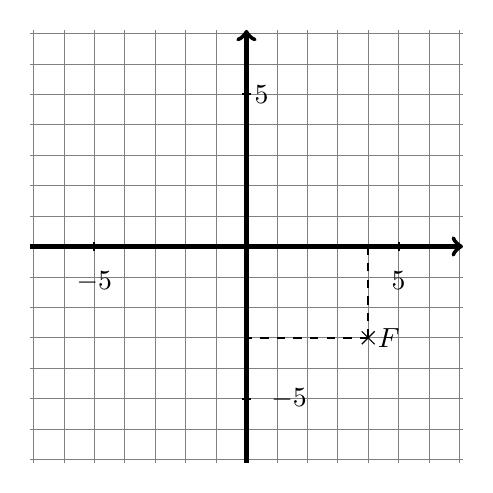
\begin{tikzpicture}[scale=0.55]
\draw[step= 20pt,gray,very thin]
(-5,-5) grid (5,5);
\coordinate (0) at (0,0);
\coordinate (1h) at (1,0);
\coordinate (2h) at (2,0);
\coordinate (3h) at (3,0);
\coordinate (4h) at (4,0);
\coordinate (5h) at (5,0);
\coordinate (6h) at (6,0);
\coordinate (-1h) at (-1,0);
\coordinate (-2h) at (-2,0);
\coordinate (-3h) at (-3,0);
\coordinate (-4h) at (-4,0);
\coordinate (-5h) at (-5,0);
\coordinate (-6h) at (-6,0);
\coordinate (1v) at (0,1);
\coordinate (2v) at (0,2);
\coordinate (3v) at (0,3);
\coordinate (4v) at (0,4);
\coordinate (5v) at (0,5);
\coordinate (6v) at (0,6);
\coordinate (-1v) at (0,-1);
\coordinate (-2v) at (0,-2);
\coordinate (-3v) at (0,-3);
\coordinate (-4v) at (0,-4);
\coordinate (-5v) at (0,-5);
\coordinate (-6v) at (0,-6);
\draw[ultra thick,->] (-5h) -- (5h);
\draw[ultra thick,->] (-5v) -- (5v);
\draw[thick] (100pt,-3pt) -- (100pt,3pt);
\draw[thick] (-100pt,-3pt) -- (-100pt,3pt);
\draw[thick] (-3pt,100pt) -- (3pt,100pt);
\draw[thick] (-3pt,-100pt) -- (3pt,-100pt);

\node[below] at (100pt,-10pt) {$5$};
\node[below] at (-100pt,-10pt) {$-5$};
%\node at (20pt,-10pt) {$\bm{1}$};
%\node at (-20pt,-10pt) {$\bm{-1}$};
\node at (10pt,100pt) {$5$};
\node[right] at (10pt,-100pt) {$-5$};

\filldraw (80pt,-60pt)  node[anchor=west] {$F$};
\draw plot[mark=x, mark options={ scale=3}] coordinates {(80pt,-60pt) };
%\filldraw (-60pt,100pt) circle (3pt) node[anchor=west] {\textbf{B}};
%\filldraw (-40pt,-80pt) circle (3pt) node[anchor=west] {\textbf{C}};
%\filldraw (-120pt,40pt) circle (3pt) node[anchor=west] {\textbf{D}};
%\filldraw (60pt,-20pt) circle (3pt) node[anchor=west] {\textbf{E}};

\draw[thick,dashed] (80pt,-60pt) -- (80pt,0);
\draw[thick,dashed] (80pt,-60pt) -- (0,-60pt);
\end{tikzpicture}
\end{center}

	}
	\end{minipage}
	\begin{minipage}[t]{0.5\textwidth}{
	\vspace{0pt}
Aide Jean et Julie à placer les points suivants sur le graphique:
\begin{tasks}[after-skip=-0.7em, before-skip=-0.7em](2)
	\task[] $G(-6;0)$
	\task[] $H(3;5 )$
	\task[] $I(2;-2 )$
	\task[] $J(-3;-2 )$
	\task[] $K(0;4 )$
  \end{tasks}
	}
	\end{minipage}}
  {1}
\end{exop}


\begin{resolu}{Un problème}{Donne la réponse au problème suivant:
\begin{center}
	{\itshape
	Je suis un nombre entier relatif compris entre $-8$ et $-11$. Ma valeur absolue est un multiple de trois. Qui suis-je~?  Donne toutes les possibilités.}
\end{center}

Solution: Les nombres entiers compris entre $-8$ et $-11$ sont $-10$ et $-9$. Le seul nombre de la liste dont la valeur absolue est un multiple de 3 est $-9$. La réponse est donc $-9$.}
{2}
\end{resolu}

\begin{exo}
 {Je suis un nombre entier relatif. Je suis supérieur à $-7$ et inférieur à $+10$. Je suis supérieur à $-15$ et inférieur à $-4$. Qui suis-je~? Donne toutes les possibilités.}
 {2}
\end{exo}
\begin{exo}
 {Je suis un nombre entier relatif compris entre $-32$ et $-39$. La somme de mes deux chiffres est 9. Qui suis-je~? Donne toutes les possibilités.}{2}
\end{exo}

\end{document}
